\documentclass{article}

\usepackage{lmodern} % Meilleure police
\usepackage[T1]{fontenc}
\usepackage[utf8]{inputenc}
\usepackage[french]{babel}
\usepackage{geometry}
\usepackage{float}
\usepackage{graphicx}
\usepackage{forest}
\usepackage{cleveref}



\geometry{left = 1.8cm, right = 1.8cm}


\begin{document}

\begin{center}
    \LARGE \textbf{Travail Pratique : MQTT - Qualité de Service (QoS) et Chiffrement TLS}
\end{center}

\tableofcontents

\newpage

\section{Introduction}

\subsection{Visualisation des logs du broker MQTT}

\noindent
Un accès SSH a été mis en place afin de permettre aux utilisateurs de consulter en temps réel les logs du broker MQTT \textbf{Mosquitto}, qui est déployé en conteneur avec \textbf{Eclipse Mosquitto}. Le broker écoute sur le port \textbf{1883} pour les connexions non sécurisées et sur le port \textbf{8883} pour les connexions chiffrées via \textbf{TLS}. Les logs du conteneur sont accessibles en se connectant au serveur via \textbf{SSH}.
\subsubsection{Connexion au serveur}

\noindent
Pour accéder aux logs, connectez-vous au serveur via SSH en utilisant les identifiants suivants :

\begin{itemize}
    \item \textbf{Utilisateur} : \texttt{mqttlogs}
    \item \textbf{Mot de passe} : \texttt{mqtt2025}
    \item \textbf{Adresse du serveur} : \texttt{hugo-serveur.cloudns.eu}
\end{itemize}

\noindent
Utilisez la commande suivante pour vous connecter :

\begin{verbatim}
ssh mqttlogs@hugo-serveur.cloudns.eu
\end{verbatim}

Une fois connecté, les logs du broker \textbf{Mosquitto} s'afficheront automatiquement en temps réel. Vous pourrez ainsi observer les connexions des clients et les messages échangés. Grâce à ces logs, il est possible de suivre en détail les échanges de données, y compris les différents paquets MQTT tels que \textbf{CONNECT}, \textbf{CONNACK}, \textbf{PUBLISH}, \textbf{SUBSCRIBE}, \textbf{PINGREQ} et \textbf{PINGRESP}, permettant ainsi d'analyser le fonctionnement du broker et le comportement des clients.

\subsubsection{Explication}  
\noindent  
Sur le serveur, un nouvel utilisateur nommé \textbf{mqttlogs} a été créé. Un script a ensuite été mis en place pour exécuter la commande suivante et afficher les logs en temps réel :  

\begin{verbatim}  
sudo docker logs -f mosquitto  
\end{verbatim}  

\noindent  
La configuration SSH de cet utilisateur a ensuite été modifiée afin qu'il exécute automatiquement ce script dès sa connexion, lui interdisant ainsi l'accès à toute autre partie du système et limitant son interaction au seul affichage des logs.

\subsection{Fichiers mis a disposition}

Plusieurs fichiers sont mis à disposition pour ce travail pratique :

\begin{itemize}
    \item \texttt{ClientMQTT\_Ping.py} : Mettre en évidence les échanges de messages \texttt{PINGREQ} et \texttt{PINGRESP}.
    \item \texttt{ClientMQTT\_QoS.py} : Tester les niveaux de qualité de service (QoS) 0, 1 et 2.
    \item \texttt{ClientMQTT\_TLS.py} : Connexion sécurisée avec TLS.
    \item \texttt{mosquitto.crt} : Certificat public pour la connexion TLS.
    \item \texttt{ClientMQTT\_Pub.py} : Simple script Python pour publier un message sur un topic.
    \item \texttt{ClientMQTT\_Sub.py} : Simple script Python pour s'abonner à un topic.
\end{itemize}

\subsection{Commandes utiles}

Lors de ce TP, vous utiliserez Wireshark pour analyser les échanges MQTT et TLS. Voici quelques filtres utiles pour faciliter l'observation des paquets pertinents.

\subsubsection{Filtres généraux}
\begin{itemize}
    \item \texttt{mqtt} : Affiche tous les paquets du protocole MQTT.
    \item \texttt{tcp.port == 1883} : Affiche uniquement les paquets circulant sur le port MQTT non sécurisé.
    \item \texttt{tcp.port == 8883} : Affiche uniquement les paquets circulant sur le port MQTT sécurisé (TLS).
    \item \texttt{tcp.port == 1883 || tcp.port == 8883} : Affiche les paquets circulant sur l'un des deux ports MQTT.
\end{itemize}

\subsubsection{Filtres spécifiques aux messages MQTT}

\begin{figure}[H]
    \centering
    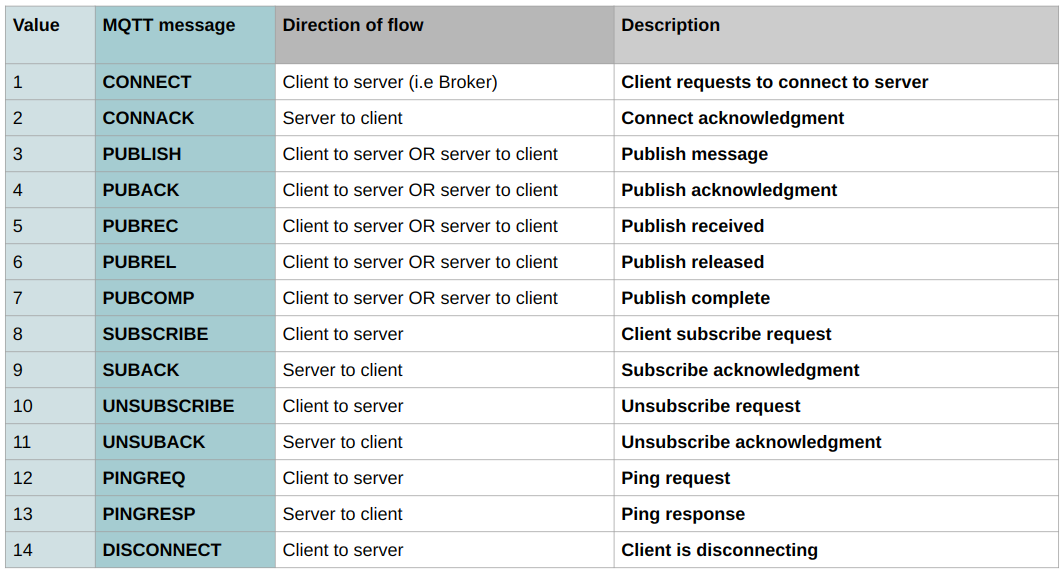
\includegraphics[width=0.8\textwidth]{Images/msgtype.png}
    \caption{Types de messages MQTT}
    \label{fig:msgtype}
\end{figure}

Ils existent plusieurs types de messages MQTT, identifiés par un numéro de type.
On peut filtrer ces messages dans Wireshark avec la syntaxe suivante :

\begin{verbatim}
mqtt.msgtype == X
\end{verbatim}

où \texttt{X} est la valeur correspondant au type de message (voir la figure \ref{fig:msgtype}).


\subsubsection{Filtres pour l'analyse TLS}
\begin{itemize}
    \item \texttt{tls} : Affiche tous les paquets du protocole TLS.
    \item \texttt{tls.handshake.type == 1} : Filtre les paquets contenant un message \textbf{Client Hello}.
    \item \texttt{tls.handshake.type == 2} : Filtre les paquets contenant un message \textbf{Server Hello}.
    \item \texttt{tls.handshake.type == 11} : Filtre les paquets contenant un \textbf{Certificat} envoyé par le serveur.
    \item \texttt{tls.record.content\_type == 23} : Affiche les paquets contenant des données applicatives chiffrées (\textbf{Application Data}).
\end{itemize}


L'ensemble de ces filtres peuvent être combinés avec des opérateurs logiques comme \texttt{AND} et \texttt{OR} pour affiner les résultats de la capture.

\section{Mise en œuvre des niveaux de qualité de service (QoS) avec MQTT}

\subsection{Objectifs}

Ce travail pratique a pour but de comprendre le fonctionnement des protocoles de qualité de service (QoS) dans le cadre de la communication MQTT. Vous utiliserez un script Python pour vous connecter à un broker MQTT et observer les différents comportements en fonction des valeurs de QoS (0, 1 et 2). 

\subsection{Pré-requis}

\begin{itemize}
    \item Accès au logs du serveur MQTT via SSH (voir section précédente).
    \item Connaissance des concepts de base de MQTT et des niveaux de QoS.
    \item Script Python mis à disposition pour simulation de la communication avec le broker.
\end{itemize}

\subsection{Connexion au Broker et Analyse des Logs}

Lancez le script Python \texttt{ClientMQTT\_QoS.py}, en choisissant un QoS de votre choix (0, 1, ou 2). Le script publiera un message et s'abonnera à un topic. 

Examinez les logs du serveur MQTT pour identifier les éléments suivants :

\begin{itemize}
    \item Le message de connexion \texttt{CONNACK} et les informations associées.
    \item Les échanges de messages lors de l'abonnement (avec \texttt{SUBSCRIBE} et \texttt{SUBACK}).
    \item Les échanges de messages pour chaque niveau de QoS (publiés avec \texttt{PUBLISH}, \texttt{PUBREC}, \texttt{PUBREL}, \texttt{PUBCOMP}).
\end{itemize}

\begin{figure}[H]
    \centering
    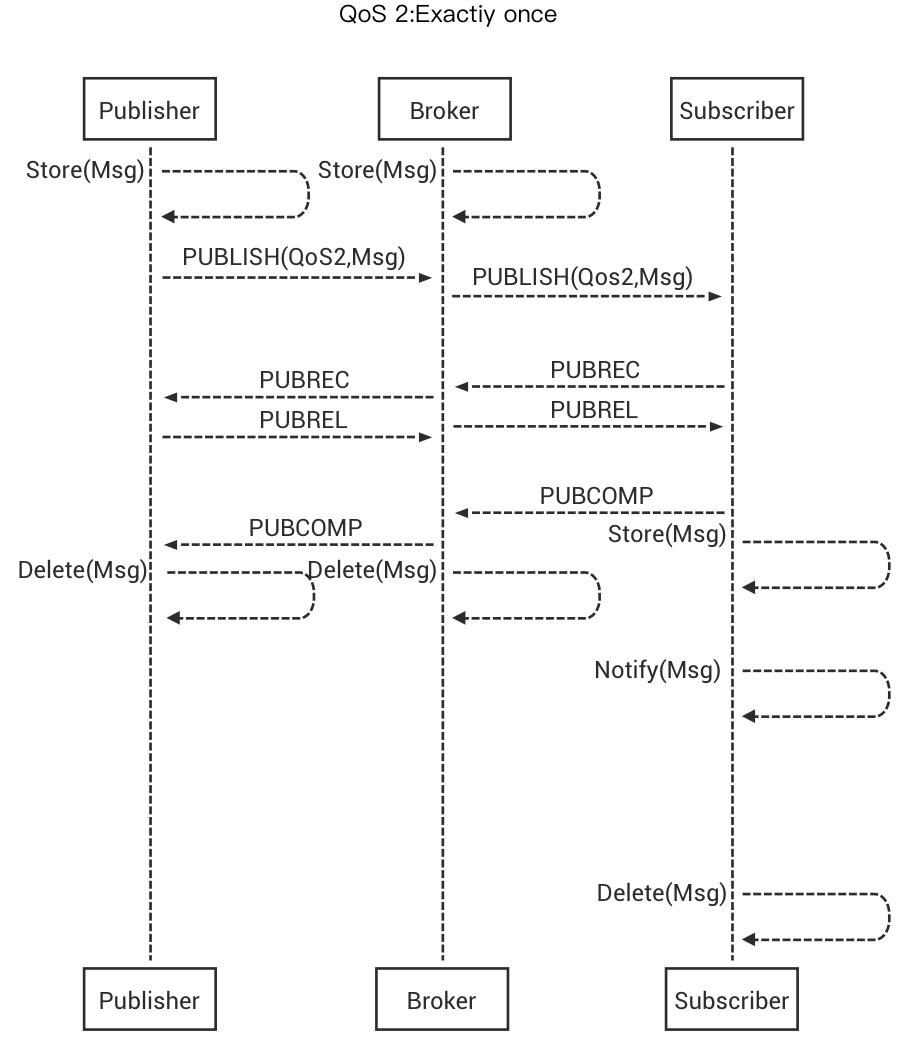
\includegraphics[width=0.6\textwidth]{Images/QoS2.png}
    \caption{Exemple d'échanges de messages avec QoS 2}
\end{figure}

\subsection{Identification des comportements selon le QoS}

En fonction du QoS sélectionné (0, 1 ou 2), analysez les différences dans les échanges et dans les messages échangés entre le client et le broker.

Répondez aux questions suivantes :

\begin{itemize}
    \item Que se passe-t-il lorsque vous utilisez QoS 0 ? Identifiez les messages échangés entre le client et le broker dans les logs.
    \item Que se passe-t-il avec QoS 1 ? Observez l'échange des messages et notez les différences par rapport au QoS 0.
    \item Que se passe-t-il avec QoS 2 ? Décrivez en détail les étapes supplémentaires de la communication (\texttt{PUBREC}, \texttt{PUBREL}, \texttt{PUBCOMP}).
\end{itemize}

\subsection{Discussion et Analyse}

Une fois l'analyse terminée, répondez aux questions suivantes :
\begin{itemize}
    \item Quelle est la différence principale entre QoS 0, 1 et 2 en termes de fiabilité et de performance ?
    \item Comment le QoS influe-t-il sur la latence et le nombre de messages échangés entre le client et le broker ?
    \item Pourquoi le QoS 2 est-il utilisé dans des cas où la fiabilité maximale est nécessaire ?
\end{itemize}

\section{Mise en œuvre des messages PINGREQ et PINGRESP avec MQTT}

Utilisez le script Python \texttt{ClientMQTT\_Ping.py}, que signifient les messages \texttt{PINGREQ} et \texttt{PINGRESP} dans le contexte de MQTT ?

Que signifient les paramètres suivants ?

\begin{itemize}
    \item \texttt{p0}, \texttt{p1}, \texttt{p2}
    \item \texttt{c0}, \texttt{c1}
    \item \texttt{kx}
\end{itemize}

Observez les logs du serveur MQTT pour identifier les échanges de messages \texttt{PINGREQ} et \texttt{PINGRESP}. Comment ces messages sont-ils utilisés pour maintenir la connexion entre le client et le broker ?

\section{Mise en évidence des parametres lors de la publication de messages avec MQTT}

Lancez le script Python \texttt{ClientMQTT\_Pub.py} pour publier un message sur un topic de votre choix. Analysez les logs du serveur MQTT pour identifier les paramètres des messages échangés.

Que signifient les paramètres suivants ?
\begin{itemize}
    \item \texttt{dx}
    \item \texttt{q0}, \texttt{q1}, \texttt{q2}
    \item \texttt{r0}, \texttt{r1}
    \item \texttt{mx}
\end{itemize}

Envoyez plusieurs messages à la suite sur le même topic et observez les valeurs de ces paramètres. Comment évoluent-ils à chaque message publié ?

\subsection{Paramètre retain}

Pour mettre en évidence le fonctionnement du paramètre \texttt{retain}, publiez un message sur un topic avec ce paramètre activé
et un autre message sur le même topic sans ce paramètre. Quelle est la différence entre les deux messages ?
Souscrivez ensuite à ce topic pour observer le comportement du broker dans les deux cas.


\section{Mise en œuvre du chiffrement TLS avec MQTT}

\subsection{Introduction : Le chiffrement TLS}

Le protocole TLS (Transport Layer Security) sécurise les communications réseau en garantissant la confidentialité, l'intégrité et l'authenticité des échanges. Il repose sur une paire de clés : une clé privée (\texttt{mosquitto.key}), conservée sur le serveur, et un certificat public (\texttt{mosquitto.crt}), distribué aux clients.

Lorsqu'un client se connecte, il envoie un message \textbf{Client Hello} (TLSv1.3). Le serveur répond avec un \textbf{Server Hello} accompagné de son certificat. Si celui-ci est valide, une clé de session est générée pour chiffrer toutes les communications MQTT.

Pour les plus curieux, voici un super site qui illustre les échanges TLS 1.3: \texttt{https://tls13.xargs.org/}

\subsection{Mise en place et analyse}

Le broker Mosquitto est configuré pour écouter sur le port \textbf{8883}, avec les certificats TLS déjà générés et en place.

\bigskip
\noindent
\textbf{Connexion d'un client Python sécurisé} \\
Le script client doit utiliser la fonction \texttt{tls\_set()} pour spécifier le certificat \texttt{mosquitto.crt}, qui est auto-signé (généré par vous-même et non par une autorité reconnue comme Let's Encrypt). Ce certificat doit être accessible au client pour établir une connexion sécurisée via TLS, en vérifiant le serveur.

\bigskip
\noindent
\textbf{Analyse du chiffrement avec Wireshark} \\
En capturant le trafic sur le port \textbf{8883}, il est possible d'observer les échanges TLS : identification des messages \textbf{Client Hello} et \textbf{Server Hello}, ainsi que la transformation des messages MQTT en \textbf{Application Data} chiffrée.

\subsection{Analyse et compréhension}

Quelques questions permettent de valider la compréhension du chiffrement TLS : \begin{itemize} \item Quels sont ses objectifs ? \item Que contient le message \textbf{Client Hello} ? \item Comment s’assurer que la communication MQTT est bien chiffrée ? \item Pourquoi Wireshark ne peut-il plus lire le contenu des messages MQTT ? \end{itemize}

\section{Mise en oeuvre d'un environnement complet avec MQTT}

Nous allons simuler un environnement d'une maison connectée avec plusieurs capteurs.
La hiérarchie des topics est représentée dans l'arbre suivant :

\begin{center}
    \begin{forest}
    for tree={
        font=\ttfamily,
        grow'=0,
        edge={->},
        l sep=40mm
    }
    [
    maison
    [chambre\_1
        [temperature, label=right:QoS 0]
        [humidite, label=right:QoS 0]
        [mouvement, label=right:QoS 2]
        [qualite-air, label=right:QoS 1]
    ]
    [chambre\_2, label=right:{(idem)}]
    [sdb, label=right:{(idem)}]
    [salon, label=right:{(idem)}]
    [cuisine, label=right:{(idem)}]
    [terrasse
        [luminosite, label=right:QoS 0]
        [humidite, label=right:QoS 0]
    ]
    [jardin, label=right:{(idem)}]
    [pluie, label=right:QoS 1]
    ]
    \end{forest}
\end{center}

Ces topic représentent les différents capteurs de la maison connectée. Chaque capteur publie des informations sur son topic respectif. 
Par exemple :
\newline
Si on veut souscrire à la température de la chambre 1, on souscrit au topic \texttt{maison/chambre\_1/temperature}.
\newline
Si on veut toute les informations du salon, on souscrit au topic \texttt{maison/salon/\#}.
\newline
Si on veut les informations de tous les capteurs de la maison, on souscrit au topic \texttt{maison/\#}.
\newline
Si on veut les informations de toutes les températures de la maison, on souscrit au topic \texttt{maison/+/temperature}.


\subsection{Question}
Mettre en oeuvre quelques commandes pour comprendre le fonctionnement des \# et des + dans les topics MQTT.


\end{document}

